\chapter{Influence of fluid dynamics of the system on the extracted power}

\section{Introduction}

Galloping occurs as a result of the pressure difference created due to the relative distance between the shear layers and the respective walls of the cross section, at the top and bottom sides of the body. As discussed in section \ref{subsec:c_y and shear layers}, the instantaneous induced angle makes one of the separated shear layers closer to the wall creating a low pressure region. This pressure difference results in a traverse forcing (normal to the direction of the flow) which becomes in phase with the transverse velocity and sustains galloping. 

From equation \ref{eqn:power_alt} discussed in section \ref{subsec:ave_pow} it is clear that the power transferred from fluid to the body is a function of the induced forcing $F_y$ and the transverse velocity $\dot{y}$. The sign of the average power represents the direction of power transfer where the $+$ ve sign represents the power transfer from fluid to the body and $-$ ve being power transferring from body to the fluid. 

Thus, then  according to equation \ref{eqn:power_alt} it can be deduced that if there is a scenario where both high induced forcing and high transverse velocities are present, higher power output could be achieved. This brings to the analysis of the $C_y$ vs. $\theta$ curve. \citet{Luo1994}, showed that the afterbody of the cross section has a direct impact on $C_y$ vs. $\theta$ curve. One interesting observation of this study was that delaying the shear layer re-attachment results in higher peak induced force coefficient $C_y$ occurring at high induced angles (high transverse velocities).    

Therefore, it could be hypothesised that a higher power transfer could be obtained by delaying the shear layer re-attachment. 

Here, the influence of shear layer and its reattachment on the mean power is studied by introducing a cross section which is a hybrid of a square and a triangle. The cross section is transformed gradually by manipulating the ratio of two length scales.

The stationary forcing data are presented for each cross section followed by the QSS power curves. Based on the QSS power data, an optimum cross section for power extraction is identified. As a negative region on some $C_y$ vs. $\theta$ curves were observed, the underpinning reason for this region was investigated through an analysis of the surface pressure and flow velocity data. The results and discussion of this analysis are presented. Following this, a comparison is made between QSS and DNS mean power at on the cross section which provides an optimum mean power.       

A final summary is presented explaining the influence of the behaviour of the shear layer on mean power output and the preliminary design considerations to optimise the fluid mechanics to obtain an optimum power output. 

\section{Influence of the shear layers}

In a typical cross section which sustains galloping, the induced lift \cy\ increases with increasing induced angle $\theta$ until it reaches a maximum value of \cy where the shear layer re attachment occurs. The lift force then decreases as $\theta$ is further increased. The underlying mechanism for this behaviour is discussed in detail in section \ref{subsec:c_y and shear layers}.   

\subsection*{Selection of the cross section}

\begin{figure}[!h]
\setlength{\unitlength}{\textwidth}

  \begin{picture}(1,0.36)(0,0.74)
    
  \put(0.2,0.76){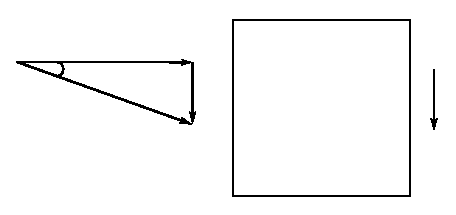
\includegraphics[width=0.5\unitlength]{./chapter-literature-revirw/fnp/setup-1.eps}}         
      
      
   
 	\put(0.315,1.04){$U$}
 	\put(0.3,0.95){$U_i$}
    \put(0.42,1.0){$\dot{y}$}
    \put(0.28,1.003){ $\theta$}
    \put(0.7,0.99){\small $(+)$}
      	

 	
 	 

     

  \end{picture}

 \caption{Induced angle of attack on a square prism due to the resultant of free-stream velocity of the fluid and transverse velocity of the body.}
    \label{fig:induced_lift_sketch}
\end{figure}

The cross section selected to test the shear layer influence on power was a hybrid cross section of a square and a triangle or in other words a pentagon which is illustrated in figure \ref{fig:hybrid_section}. This was produced by systematically tapering off the trailing edges of the top and bottom sides of the square cross section. The $\ratio$ was changed gradually from 1 to zero at increments of 0.25 where 1 being the square cross section and 0 being an isosceles triangle. This type of a cross section was selected because after analysing the shear layer behaviour of a galloping body it was found out that it is crucial to have the afterbody and the shear layer close to the body. And therefore the presence of the horizontal part of the top and bottom sides of the cross section. Rectangular cross sections are not very suitable as it may have a earlier shear layer re-attachment \citet{Paidoussis2010}. Another option was to use trapeziums as \citet{Luo1994}. However, the initial shear layers are quite far away and thus, maybe difficult to initialise galloping. The main focus was to study influence of shear layer behaviour on galloping, and thus the current hybrid cross section was used to study this behaviour by systematically delaying the shear layer reattachment of the initial square cross section. 

\section{Static body results}
\label{sec:cross-sec-Static body results}
\begin{table}[ht]

\begin{center}
\setlength{\unitlength}{\textwidth}

\begin{tabular}{c c c c c} % centered columns (4 columns)
\hline\hline %inserts double horizontal lines
\\[0.2ex]
$\ratio$ & $a_1$ & $a_3$ & $a_5$ & $a_7$ \\ [0.8ex] % inserts table 
%heading
\hline 

\\[0.8ex]% inserts single horizontal line
$0$ &  -2.30617 & -269.075 & -59.2929 & 4.74389\\[0.8ex]
    & -5.08342 & -56.5390e & -160.505e & -105.773\\[0.8ex]
    &  4.40685 & 19.9213 & 22.8894 & 7.68556\\[1ex]


\\[0.8ex]% inserts single horizontal line
$0.25$ & -0.605146 & -19.4346 &-82.4463 & -94.4226\\[0.8ex]
      & 2.50538 & 9.91021  & 10.2712 & 3.94112 \\[1ex]

 \\[0.8ex]% inserting body of the table


 $0.5$ & 1.44734 & 4.83885  & -166.900e & -983.072 \\[0.8ex]% inserting body of the table
  & 1.51455e & 15.8476 & 52.5465 & 62.8067 \\ [1ex] % [1ex] adds vertical space
  
  \\[0.8ex]% inserting body of the table
  
   $0.75$ & 1.76938 & 35.2630 & -345.562 & -10072.7 \\[0.8ex]
          & 1.77553 & 43.0120 & 262.983 & 638.484 \\ [1ex]
          
          
  
  
\hline %inserts single line


\end{tabular}

\caption{Coefficient values used in the 7th order interpolation polynomial at $Re=200$. Data present for $\ratio=0-0.75$ at increments of $0.5$. Multiples polynomials were used to attain a better fit. The plot of the compound fit is presented in figure \ref{fig:lift_curves-hybrid}.} 
 
\label{table:cy-coefficients-hybrid} % is used to refer this table in the text
\end{center}
\end{table}



Stationary time averaged $C_y$ results were obtained for cross sections where $\ratio=1,0.75,0.5,0.25$ and $0$ using DNS at $\reynoldsnumber=200$. Where $\ratio=1$ being the square and $\ratio=0$ being an isosceles  triangle. Table \ref{table:cy-coefficients-hybrid} shows the coefficients of the $7^{th}$ order curve fitting for each cross section. In order to achieve a better fit, piecewise interpolation using multiple $7th$ order polynomials were incorporated for a single cross section. During the curve fitting process more importance was given for accurately fitting  the positive portion of the $C_{y}$ curve, as the power transfer from the fluid to the body occur in this region. 

\begin{figure}
  \setlength{\unitlength}{\textwidth}

  \begin{picture}(1,0.75)(0,0)
    % % %90
      % % % Parkinson Data 
      \put(0.035,0.5){\includegraphics[width=0.5\unitlength]{./chapter-cross-sections/fnp/lift_curve_sq.eps}}
      \put(0.495,0.5){\includegraphics[width=0.5\unitlength]{./chapter-cross-sections/fnp/lift_curve_075.eps}}
      \put(0.035,0.27){\includegraphics[width=0.5\unitlength]{./chapter-cross-sections/fnp/lift_curve_05.eps}}
      \put(0.495,0.27){\includegraphics[width=0.5\unitlength]{./chapter-cross-sections/fnp/lift_curve_025.eps}}
      \put(0.3,0.0){\includegraphics[width=0.5\unitlength]{./chapter-cross-sections/fnp/lift_curve_tri.eps}}
      
      
   
      
      
%      \put(0.23,0.00){ $\displaystyle\frac{c}{\rho\mathcal{A}U}$}
%      \put(0.73,0.00){ $\displaystyle\frac{c}{\rho\mathcal{A}U}$}

      \put(0.3,0.26){$\theta$}
      \put(0.76,0.26){$\theta$}
      \put(0.56,-0.01){$\theta$}
      
      \put(0.01,0.405){$\displaystyle C_y$}
       \put(0.01,0.65){$\displaystyle C_y$}
      \put(0.3,0.14){$\displaystyle C_y$}
      
      \put(0.106,0.705){\small(a)}
      \put(0.565,0.705){\small(b)}
      \put(0.106,0.475){\small(c)}
      \put(0.565,0.475){\small(d)}
      \put(0.37,0.207){\small(e)}
      

  \end{picture}

  \caption{Induced lift coefficient $C_y$ at different angles for selected cross sections. Data presented for cross sections, (a) square, (b) $\ratio=0.75$, (c) $\ratio=0.5$, (d) $\ratio=0.25$ and (e) triangle.}
  \label{fig:lift_curves-hybrid}
\end{figure} 

The $C_y$ vs. $\theta$ curves in figure \ref{fig:lift_curves-hybrid} shows that the peak value of \cy\ shifts to the right as $\ratio$ is increased, hence, the peak \cy\ occurs at high induced angles.  These data agree with \citet{Luo1994} where the peak of the maximum \cy\ value was shifted to higher induced angles when reattachment was delayed. As $\theta$ is proportional to the transverse velocity of the body $\tan{\theta}=\frac{\dot{y}}{U}$, the peak value of \cy\ occurs at high induced velocities as \ratio\ is decreased. A negative region of $C_y$ vs. $\theta$ curves on cross sections where $\ratio\geq0.25$. Here, initially \cy\ decreases as $\theta$ is increased and the increases after reaching a minimum. The presence of this negative portion is an indication of unfavourable power transfer, i.e. power transferred from body to the fluid as the direction of the force and velocity vectors are out of phase. This will be further discussed in the upcoming sections of this chapter.    

 
 
 \section{QSS Mean power output}
 \label{sec:cross-sec-qss-mean power}
 
 % !TeX spellcheck = en_GB
\begin{figure}[!htb]
  \setlength{\unitlength}{\textwidth}

        \begin{picture}(1,0.4)(-0.02,0)

 
      
      \put(0.08,0.02){\includegraphics[width=0.75\unitlength]{./FnP/mean_power_hyb.eps}}

      \put(0.46,0.00){\massdamp}
      
      
     
       \put(0.03,0.235){$\displaystyle\frac{P_{m}}{\rho \mathcal{A}U^3 }$}
      

      %\put(0.095,0.218){\small(a)}
      %\put(0.565,0.218){\small(b)}
      
    \end{picture}

  \caption{Dimensionless mean power obtained using QSS model as a function of \massdamp. Data presented for five selected cross sections, square ($\triangle$), $\ratio=0.75$ (+), $\ratio=0.5$ (\ding{117}), $\ratio=0.25$ ($\times$) and triangle (\ding{108}) at $\reynoldsnumber=200$, $\massstiff=100$.}
    \label{fig:power_curves}
\end{figure}

 %vspace{10cm}

 
 Mean power output predictions could be obtained for these different cross sections using the QSS model and the stationary induced lift data obtained earlier using as inputs to the QSS model. Figure \ref{fig:power_curves} shows the mean power \massdamp\ vs. mean power for different cross sections namely $\ratio=1,0.75,0.5,0.25 \text{and} 0$. The maximum mean power increases until $\ratio=0.25$. This agrees well with the formulated hypothesis. The shear layer re-attachment is delayed as \ratio\ is decreased and an increase in maximum power output could be observed. As \ratio\ is further decreased to $\ratio=0$ the peak mean power output is reduced. This result goes against the initial hypothesis. Thus, it was further investigated the cause of this reduction in mean power output. 
 
As the presented power data were obtained from the QSS model, the reason for the power reduction at $\ratio=0$ could be identified through the main energy input of this model, which is the induced forcing. It was identified in section \ref{sec:cross-sec-Static body results} the presence of a negative portion of the $C_y$ vs. $\theta$ curve at $\ratio\leq0.25$. It was established in that section that the presence of this negative portion of the $\cy$ vs. $\theta$ curve results in unfavourable power transfer i.e. power transfer from the body to the fluid. By further analysing the lift curves in figure \ref{fig:lift_curves-hybrid} (d) and (e), it could be clearly observed that the negative region of the curve increases as \ratio\ is decreased. An argument could be that when \cy\ becomes negative it will preclude galloping altogether. This argument is partially true. However, manipulating the initial condition (initial transverse velocity) will somewhat rectify this problem. If an initial velocity which would make a positive induced angle is given galloping would sustain. This is how the mean power data were obtained for $\ratio=0.25$ and $\ratio=0$. That being mentioned to sustain galling another crucial factor is damping \citet{Paidoussis2010}. This is the reason why even though a higher initial condition is given the bandwidth of \massdamp\ for power production is short for $\ratio=0.25\ \text{and}\ 0$ compared to other tested cross sections. 

\section{Presence of the negative region of the $\cy$ vs. $\theta$ curves}

As a reduction in power was observed in some cross sections due to the presence of a negative portion of the $\cy$ vs. $\theta$, further investigations were carried out in order to understand the underlying reasoning for this phenomenon.

\subsection{Surface pressure}
\label{subsec:cross-sec-surface pressure}

As the driving force of the galloping body is the pressure forces created from the relative distances of the shear layers, the primary investigation was carried out analysing surface pressure data on the time averaged stationary data of the cross section. The test cross section taken here out of the cross sections was the isosceles triangle ($\ratio=0$) as it produced the largest negative region out of the cross sections tested for mean power output. 

Time averaged (to filter out the influence of vortex shedding) surface pressure data  on the top and bottom surfaces of the cross sections at $\theta=4^{\circ}$, $\theta=16^{\circ}$ and $\theta=21^{\circ}$ were obtained for the isosceles triangle. By having a closer look at the \cy\ vs. $\theta$ curves it could be seen that these points correspond to a negative \cy\ that is further decreasing with increasing $\theta$, a negative \cy\ that is increasing with increasing $\theta$ and a significantly positive value of \cy.        
 
 
\begin{figure}
  \setlength{\unitlength}{\textwidth}

        \begin{picture}(1,1.1)(0,0.35)

      % % % Parkinson Data 
      \put(0.1,1.1){\includegraphics[width=0.75\unitlength]{./chapter-cross-sections/fnp/surf-pres-tri-4.eps}}
      \put(0.1,0.737){\includegraphics[width=0.75\unitlength]{./chapter-cross-sections/fnp/surf-pres-tri-16.eps}}
      \put(0.1,0.38){\includegraphics[width=0.75\unitlength]{./chapter-cross-sections/fnp/surf-pres-tri-21.eps}}
     
      
      



%      
    \put(0.21,1.41){\small(a)}
     \put(0.21,1.05){\small(b)}
     \put(0.21,0.69){\small(c)}
\put(0.1,0.95){$\displaystyle P_{s}$}
\put(0.1,1.3){$\displaystyle P_{s}$}
\put(0.1,0.56){$\displaystyle P_{s}$}
\put(0.26,0.35){Relative destance from the leading edge}

      
    \end{picture}

    \caption{Surface pressure of top (\ding{83}) and bottom (\ding{117})  surfaces of the static triangular cross section at (a) $\theta=4^\circ$, (b) $\theta=16^\circ$ \ and (c) $\theta=21^\circ$ A clear pressure difference is visible between the surfaces. The top surface comparatively has more negative pressure where a lift is created which results in a negative $C_y$ at $4^\circ$ and reduces as $\theta$ \ is increased, while the vice versa occurs at the top surface.}
    \label{fig:surf_pres}
\end{figure}

 %vspace{10cm}
 
 
 
Figure \ref{fig:surf_pres} shows the surface pressure of the top and bottom surfaces of the body ($\ratio=0$) starting from  the leading edges. At $\theta=4^{\circ}$, the pressure of the bottom of the body is grater than the top. Therefore, a pressure difference is created and a force is generated in the upward direction which according to the sign convention presented in \ref{fig:induced_lift_sketch}, is against the velocity of the body, hence giving a negative $\cy$. As $\theta$ (figure \ref{fig:surf_pres} (b)) is increased, to $16^{\circ}$ the gap between the surface pressure at the leading edge between the top and the bottom reduces. This effect results in the increase in $\cy$ (although it is still in the negative region). As $\theta$ is further increased at $21^{\circ}$ (figure \ref{fig:surf_pres} (c)) the surface pressure on the top side becomes grater than the bottom. Therefore, the net effect of the pressure difference is a positive $\cy$ which the driving force $F_y$ in phase with the velocity of the body.

\subsection{Velocity profiles at the points of flow separation}

The most important points of a cross section under galloping are the two flow separation points of the leading edges of the cross section, where a significant pressure difference occur. A key variable which directly relates to the fluid dynamic pressure is the velocity of the fluid. Although not strictly true in all cases of viscous flows, one should expect that a higher flow speed correspond with a lower pressure from basic fluid dynamic theory. A clearer picture could be obtained by analysing the flow velocity behaviour at the separation points in order to identify the cause of the pressure differences occurred at the leading edges.

\begin{figure}[!htb]
\setlength{\unitlength}{\textwidth}

  \begin{picture}(1,0.38)(0,0.74)
    
  \put(0.32,0.76){\includegraphics[width=0.32\unitlength]{./chapter-cross-sections/fnp/tri-sketch.eps}}         
      
      
   
 %	\put(0.28,0.937){$\theta$}
 	%\put(0.52,0.74){$l$}
   

 	
 	 

     

  \end{picture}

 \caption{Illustration of the lines along which the flow velocity magnitudes have been extracted. The data have been extracted along a line starting from the separation points in the outward direction (shown with arrows) for the top and bottom surfaces.}
    \label{fig:tri-sketch}
\end{figure}
   
Velocity magnitude data of the flow were obtained along two lines parallel to the front wall of the cross section one stating at the top and the other stating at the bottom leading edges of the cross section spreading outward as illustrated in figure \ref{fig:tri-sketch}. The lengths of these lines were equal to the width of the cross section. Data were obtained for the same cases presented earlier i.e. isosceles triangle ($\ratio=0$) at $\theta=4^{\circ}$, $\theta=16^{\circ}$ and $\theta=21^{\circ}$.
       
\begin{figure}[!h]
  \setlength{\unitlength}{\textwidth}

        \begin{picture}(1,1.1)(0,0.35)

      % % % Parkinson Data 
      \put(0.1,1.1){\includegraphics[width=0.75\unitlength]{./chapter-cross-sections/fnp/vel_prof-tri-4.eps}}
      \put(0.1,0.737){\includegraphics[width=0.75\unitlength]{./chapter-cross-sections/fnp/vel_prof-tri-16.eps}}
      \put(0.1,0.38){\includegraphics[width=0.75\unitlength]{./chapter-cross-sections/fnp/vel_prof-tri-21.eps}}
     
      
      



%      
    \put(0.21,1.41){\small(a)}
     \put(0.21,1.05){\small(b)}
     \put(0.21,0.69){\small(c)}
\put(0.1,0.95){$\displaystyle V_m$}
\put(0.1,1.3){$\displaystyle V_m$}
\put(0.1,0.56){$\displaystyle V_m$}
\put(0.34,0.35){Distance from the leading edge}

      
    \end{picture}

    \caption{Velocity magnitudes of the flow along a line parallel to the front surface spreading towards top (\dashedrule) and bottom (\solidrule) boundaries (figure \ref{fig:tri-sketch}). These two lines (for the top and bottom surfaces) start from the top and bottom leading edges of the triangular cross section. Data present (a) $\alpha=4^\circ$, (b) $\alpha=16^\circ$ \ and (c) $\alpha=21^\circ$.}
    \label{fig:vel-profile}
\end{figure}

 %vspace{10cm}


The velocity profiles at the chosen three incident angles are presented in figure \ref{fig:vel-profile}. A sudden rise of velocity magnitude could be observed at the flow separation points. The velocity magnitude at the top separation point  at $\theta= 4^{0}$ (figure \ref{fig:vel-profile} (a)) is higher than the bottom separation point, leading to a lower pressure at the top edge. However, the velocity magnitude at the bottom edge becomes grater than the top edge at $\theta=16^{\circ}$. The difference between the top and bottom velocity magnitude at the separation points tends to increase as $\theta$ is increased to $21^{\circ}$, where the velocity magnitude at the bottom being grater than the top (figure \ref{fig:vel-profile} (c)). This effectively creates the pressure difference created in figure \ref{fig:surf_pres} (c), which leads to a positive \cy\ and results in a forcing which is in phase with the velocity of the body. 

 
\begin{figure}[t!]

  \setlength{\unitlength}{\textwidth}

  \begin{picture}(1,0.35)(0,0.725)

    \put(-0.01,0.76){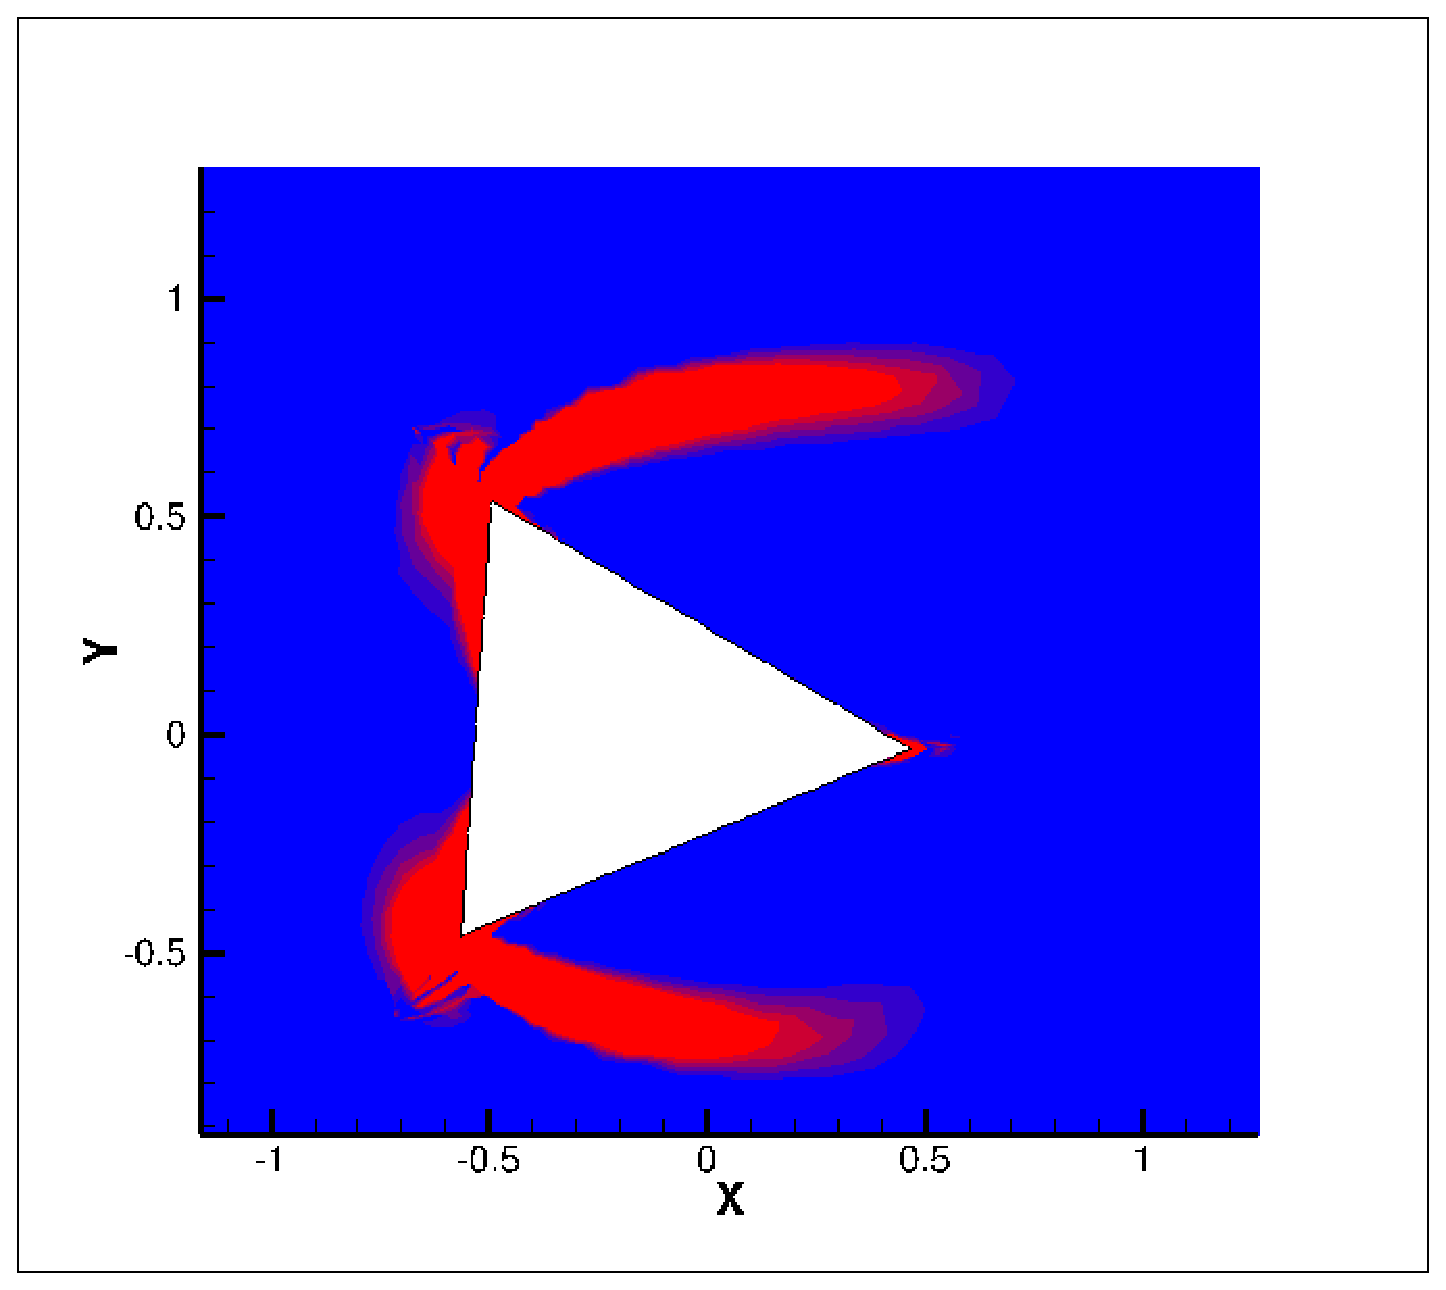
\includegraphics[width=0.33\unitlength]{./chapter-cross-sections/fnp/4.eps}}
    \put(0.335,0.76){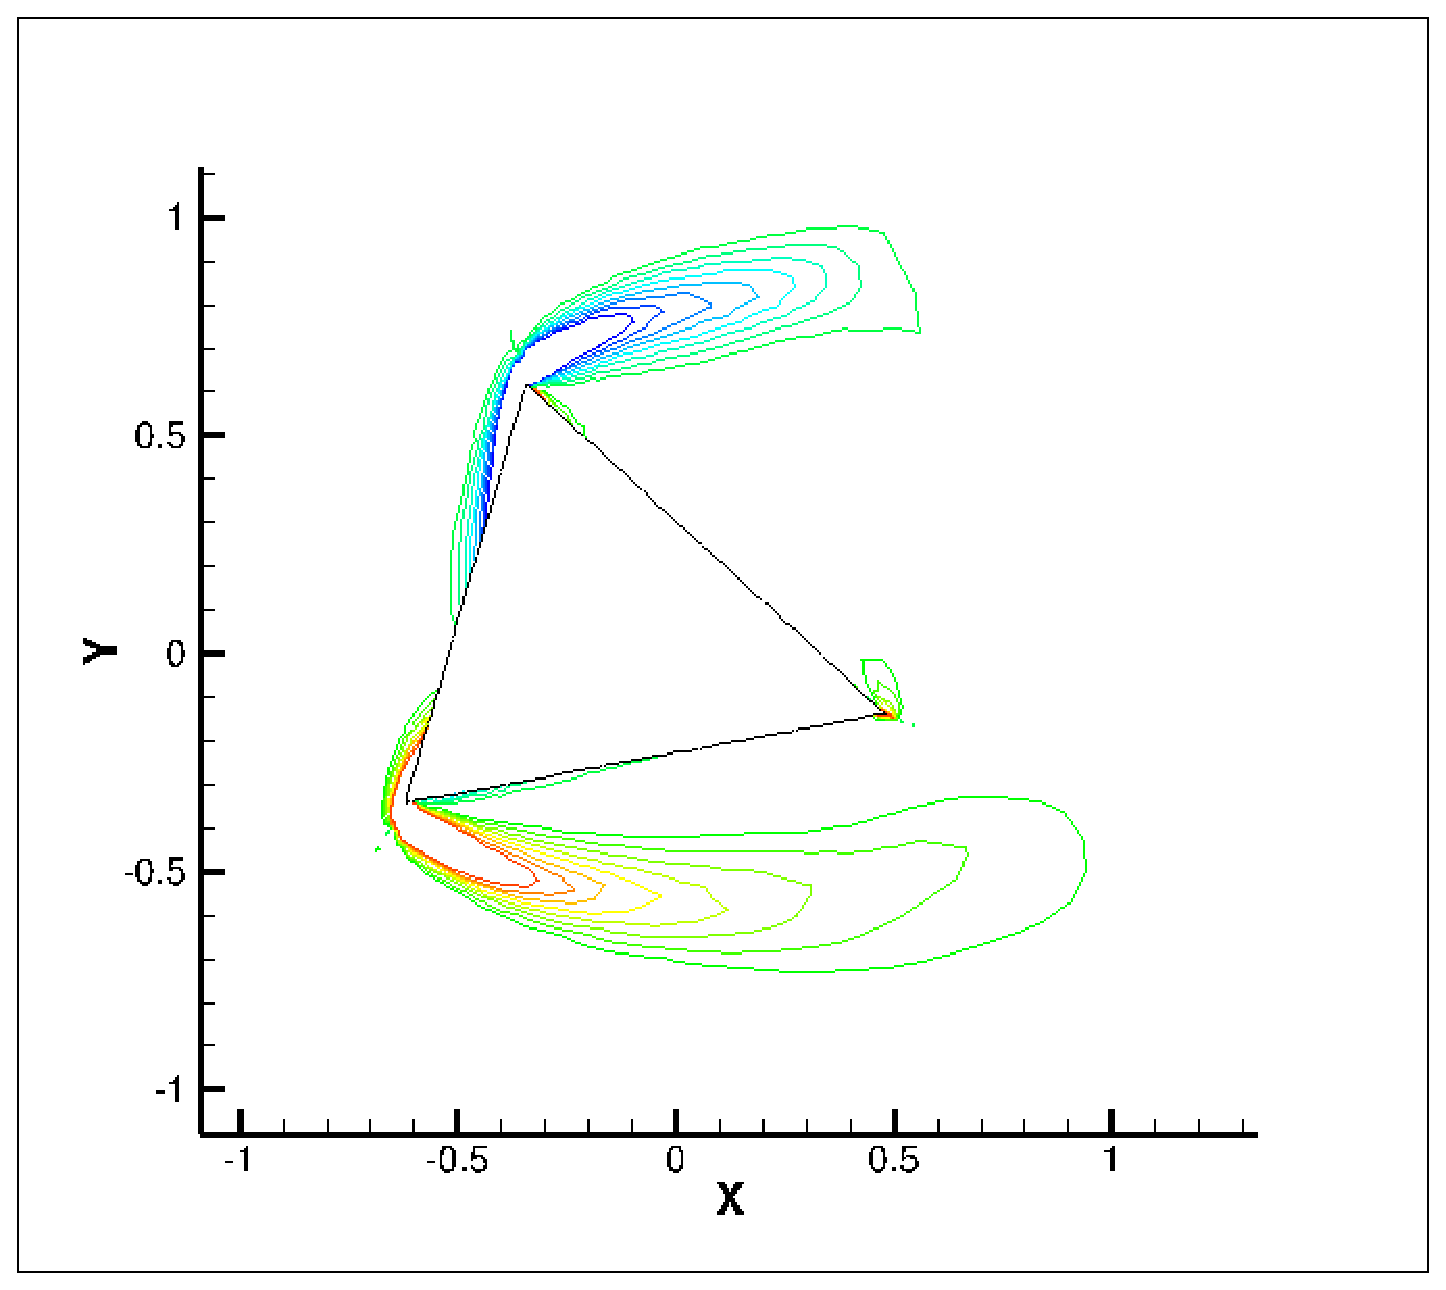
\includegraphics[width=0.33\unitlength]{./chapter-cross-sections/fnp/16.eps}}
    \put(0.68,0.76){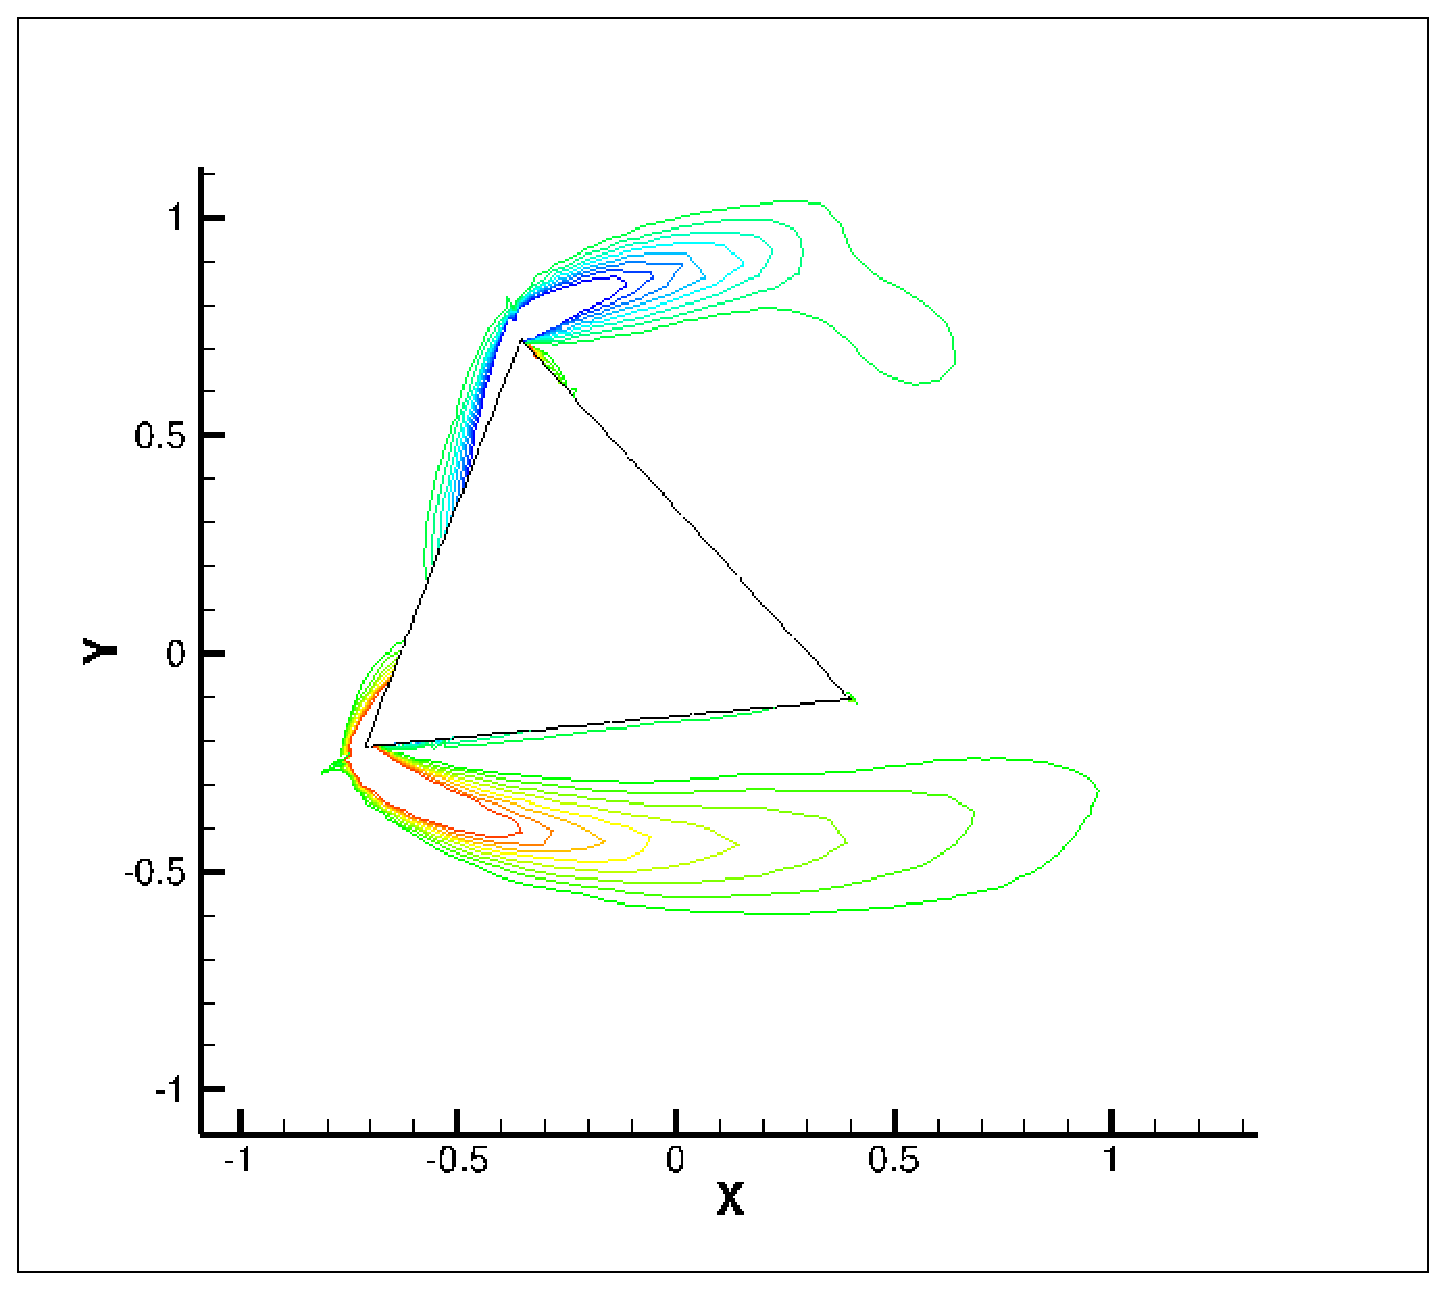
\includegraphics[width=0.33\unitlength]{./chapter-cross-sections/fnp/21.eps}}

   
    
    \put(0.0,0.735){(a)}    
    \put(0.34,0.735){(b)}
    \put(0.685,0.735){(c)}
  
  \end{picture}

  \caption{Contours of the magnitude of the shear strain rate of time averaged flow field on the  stationary isosceles triangle ($\ratio=0$) at $\reynoldsnumber=200$ at different incidence angles. (a) $4^{\circ}$ ( negative value of \cy\ that is further decreasing with increasing $\theta$), (b) $16^{\circ}$ ( negative value of \cy\ that is increasing with increasing $\theta$) and (c) $21^{\circ}$ $\theta$ and a significantly positive value of \cy. The bottom shear layer comes closer to the bottom wall and as the angle of incidence increases.}
  \label{fig:triangle-shear_layers}
\end{figure}




  


The stream functions of the time averaged flow-filed of the stationary isosceles triangle at  $\theta=4^{\circ}$, $\theta=16^{\circ}$ and $\theta=21^{\circ}$ are presented in figure \ref{fig:triangle-shear_layers}. Here, it could be observed that the proximity of the bottom shear layer increases as $\theta$ is increased from $4^{\circ}-21^{\circ}$.

By comparing the pressure and the velocity plots together with the stream function flow-field data, it could be seen \cy\ is governed by two mechanisms. Initially at $\theta= 4^{0}$ an un even distribution of the flow is created due to the profile and the positioning (angle of attack) of the geometry creating a forcing ($F_{y}$) similar to the generation of lift of an aerofoil. Comparing figure \ref{fig:triangle-shear_layers} (a) to (b) and (c) the proximity of the bottom shear layer low and hence, does not create a significant pressure force form the relative proximities of the top and bottom shear layers. Therefore, the aerofoil effect becomes more dominant.  

As $\theta$ is increased from $\theta=16^{\circ}$ to $21^{\circ}$, the proximity of the bottom shear layer to the wall of the body increases (figure \ref{fig:triangle-shear_layers} (b) and (c)), and thus becoming the more dominant forcing of the system. This uneven flow distribution as discussed earlier and in \ref{subsec:c_y and shear layers}in detail, creates the positive region of the \cy\ vs. $\theta$ curve.



    
 
 
 
 
 



